\section{Introduction}

The Zeeman effect was first observed in 1896 by the Dutch physicist Pieter Zeeman. Although at first there was no clear explaination
for the results, the experiment was a cornerstone in proving the existence of electron Spin and magentic moments.

The Zeeman effect is the splitting of spectral lines in the presence of a magnetic field. The effect is caused by the
interaction of the magnetic field with the magnetic moment of the electron.

It is important to point out that the Zeeman effect does not occur in all cases. For example, a simple case where it does not occur
is in the ground state of the Helium atom, where the electrons are paired and the total magnetic moment is zero, as both atoms occupy the 1s orbital,
and have opposite spin (remember also that the s orbitals do not have any orbital angular momentum, becuase the only possible l
quantum number is l=0).

In this experiment, we will be using a Hg-Cd lamp to observe the Zeeman effect. The electron for Mercury (Hg) is given by: $[Xe] 4f^{14} 5d^{10} 6s^2$, and the
configuration for Cadmium (Cd) is given by: $[Kr] 4d^{10} 5s^2$

All of the orbitals of these are filled, the spin magnetic moments inside the orbitals will cancel out,
and we can safely ignore the effect of spin in spectral line separation. The report will then be scoped to the
\textbf{Normal Zeeman Effect}.

In order to set the foundation for the experiment, we will have to go back to electromagnetism.
We can consider the electron as a point charge, with a charge of $-e$, and a mass of $m_e$ travlling around the
charged nuclus.

A torque given by $\tau = \vec{\mu} \times \vec{B}$ will be applied to the electron, where $\vec{\mu}$ is the
magnetic moment of the electron,
and is given by $\vec{\mu} = \gamma \vec{L}$, where $\gamma = - \frac{e}{2 m_e}$ is the gyromagnetic ratio,
and $\vec{L}$ is the orbital angular momentum of the electron.

Given this information, we can now calculate the energy shift of the electron in the presence of a magnetic field.

\begin{equation}
    \Delta E = - \vec{\mu} \cdot \vec{B} = - \gamma \vec{L} \cdot \vec{B} = - \gamma L_z B
\end{equation}

Where $L_z$ is the z component of the orbital angular momentum (assuming the field $B$ is applied in the z direction). We also know that
$L_z = m_l \hbar$, where $m_l$ is the magnetic quantum number, and $\hbar$ is the reduced Planck constant. We can rewite the above expression as:

\begin{equation}
    \Delta y = - \gamma m_l \hbar B
\end{equation}

According to this, and keeping in mind that $m_l$ can take intager values from $-l$ to $l$, we can see that the energy levels of the electron
are spaced by $\Delta E = \gamma \hbar B$. This is the energy difference between the Zeeman levels.


% Some more theoretical explaination will be needed here

The Zeeman effect can be used to estimate the value of $\frac{e}{m}$.

The change in wavelength of the spectral lines is given by:

\begin{equation}
    \Delta \lambda = \frac{\Delta S}{\Delta A} \frac{\lambda^2}{2d} \frac{2}{\sqrt[2]{\eta^2 - 1}}
\end{equation}


\begin{figure}
    \centering
    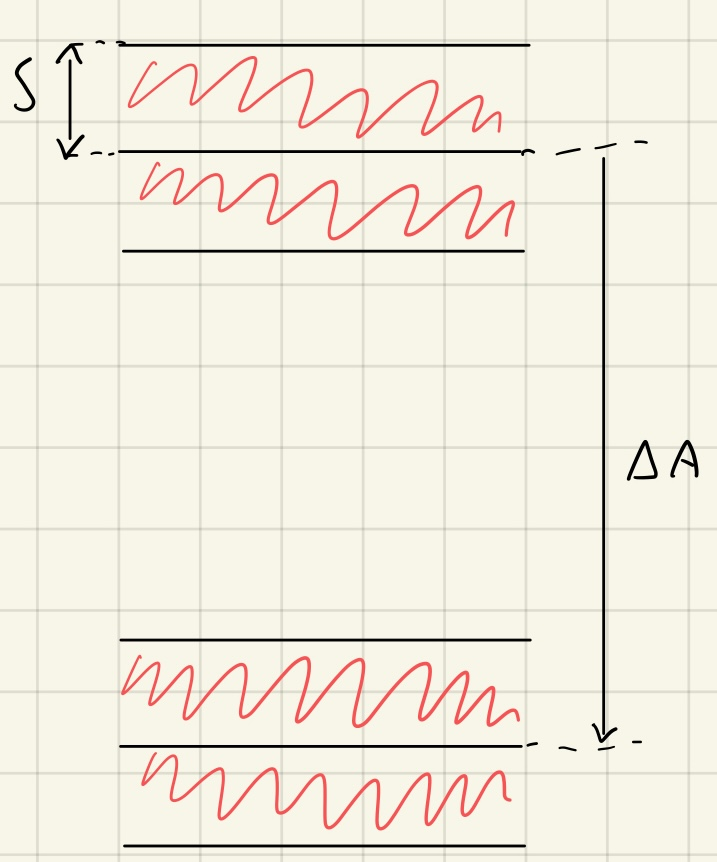
\includegraphics[width=0.8\textwidth]{intro/lambda_calc_diagram.jpeg}
    \caption{Meaning of variables in change in wavelength of spectral lines equation.}
    \label{fig:variables_lambda}
\end{figure}


Where $\Delta S$ is the separation of the zeeman split, $\Delta A$ is the separation of successive interference lines, $\lambda$ is the wavelength of the light, $d$ is the distance between the grating and the screen, and $\nu$ is the refractive index of the medium.
Figure \ref{fig:variables_lambda} helps build a better understanding of the variables involved in the equation.


We are given that the refractive index of the Lummer plate is $\nu = 1.4567$, the wavlength of the red line in cadmimum is $\lambda = 643.8 nm$, and the thickness of the Lummer plate is $d = 4.04 mm$.

Further, it can also be obtained that the change in frequency when a field is applied is given by:

\begin{equation}
    \Delta \nu = \frac{e B}{4\pi m}
\end{equation}

Where $e$ is the charge of the electron, $B$ is the magnetic field, and $m$ is the mass of the electron.

We can then use the change in frequency to estimate the value of $\frac{e}{m}$ by using $\Delta v = \frac{c}{\lambda^2} \Delta \lambda$:

\begin{equation} \label{eq:em_relationship}
    \frac{e}{m} =
    \frac{4 \pi c}{B} \frac{1}{2d\sqrt[2]{\eta^2 - 1}} \frac{\Delta S}{\Delta A}
\end{equation}

% Add stuff about polarization